% !TeX program = xelatex
\documentclass{article}
\usepackage{kotex}
\usepackage[a4paper, left=3cm, right=3cm, top=2.5cm, bottom=2.5cm]{geometry}
\usepackage{amsmath, amssymb}
\usepackage{tcolorbox}
\usepackage{caption}
\usepackage{setspace}
\usepackage{xcolor}
\usepackage{titlesec}
\usepackage{enumerate}
\usepackage{tikz}
\usetikzlibrary{arrows.meta, calc, angles, quotes}

\setstretch{1.3}
\renewcommand{\figurename}{그림}
\titleformat{name=\section,numberless}
  {\normalfont\large\bfseries\color{blue}}{}
  {0pt}{}

\title{2.10 입체 사영의 응용}
\date{}
\author{}

\begin{document}
\maketitle

\section*{2.10 입체 사영의 응용}

\subsection*{평면에서의 입체 사영}

그림 2.30은 $\mathbb{R}^2$에서 점 $(-1,0)$으로부터 $y$축으로의 입체 사영에 의한
원 $x^2+y^2=1$의 사영이다.
$(x,y)$가 원 위의 점이고 $(0,t)$가 그 사영이면,
$t$는 직선 $(-1,0)$--$(x,y)$의 기울기이므로
\begin{equation}
  t = \frac{y}{x+1} \tag{2.27}
\end{equation}

\begin{figure}[ht]
\centering
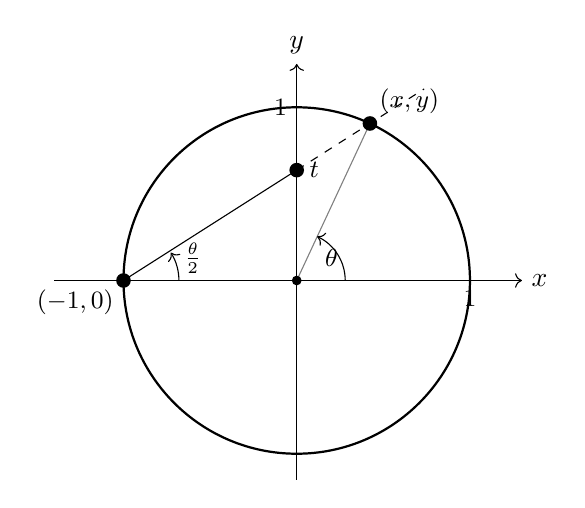
\begin{tikzpicture}[scale=2.2]
  \draw[->] (-1.4,0) -- (1.3,0) node[right] {$x$};
  \draw[->] (0,-1.15) -- (0,1.25) node[above] {$y$};
  \draw[thick] (0,0) circle (1cm);
  \def\ang{65}
  \coordinate (O)  at (0,0);
  \coordinate (N)  at (-1,0);
  \pgfmathsetmacro{\px}{cos(\ang)}
  \pgfmathsetmacro{\py}{sin(\ang)}
  \coordinate (P) at (\px,\py);
  \pgfmathsetmacro{\tv}{\py/(\px+1)}
  \coordinate (T) at (0,\tv);
  \draw[thin] (N) -- (T);
  \draw[thin,dashed] (T) -- ($(N)!1.22!(P)$);
  \draw[thin,gray] (O) -- (P);
  \fill (N) circle (1.2pt) node[below left, font=\small] {$(-1,0)$};
  \fill (P) circle (1.2pt) node[above right, font=\small] {$(x,y)$};
  \fill (T) circle (1.2pt);
  \fill (O) circle (0.8pt);
  \node[below, font=\small] at (1,0)  {$1$};
  \node[left,  font=\small] at (0,1)  {$1$};
  \draw (0.03,\tv) -- (-0.03,\tv) node[right=3pt, font=\small] {$t$};
  \draw[->,thin] (0.28,0) arc (0:\ang:0.28);
  \node[font=\small] at (0.20,0.13) {$\theta$};
  \pgfmathsetmacro{\halfang}{\ang/2}
  \draw[->,thin] (-0.68,0) arc (0:\halfang:0.30);
  \node[font=\small] at (-0.60,0.13) {$\tfrac{\theta}{2}$};
\end{tikzpicture}
\caption{평면에서의 입체 사영 (그림 2.30)}
\label{fig:2.30}
\end{figure}

$(x,y)\neq(-1,0)$을 $t$로 나타내자.
식 (2.27)로부터 $y=t(x+1)$을 원의 식에 대입하면
$(x+1)\bigl[(x-1)+t^2(x+1)\bigr]=0$이고, $(x,y)\neq(-1,0)$이므로
$x = (1-t^2)/(1+t^2)$을 얻는다.
$y=t(x+1)$에 대입하면
\begin{equation}
  (x,y) = \left(\frac{1-t^2}{1+t^2},\;\frac{2t}{1+t^2}\right) \tag{2.28}
\end{equation}

\subsection*{응용 1. 피타고라스 삼중쌍}

세 정수 $(X,Y,Z)$가 $X^2+Y^2=Z^2$을 만족할 때 \textbf{피타고라스 삼중쌍}이라 한다.
\begin{equation}
  X^2 + Y^2 = Z^2 \tag{2.29}
\end{equation}
$(Y,X,Z)$도 삼중쌍이므로 $X<Y$인 경우만, $(DX,DY,DZ)$도 삼중쌍이므로 공약수 없는 경우만 찾으면 충분하다.

$X,Y,Z$를 $(\pm1$ 이외의) 공약수 없는 정수로 가정하자.
$(X/Z)^2+(Y/Z)^2=1$이므로 $x=X/Z$, $y=Y/Z$로 놓으면 $(x,y)$는 단위 원의 유리수 점이다.
입체 사영 $t = y/(x+1)$에 의해 $t$도 유리수이므로
\begin{equation}
  t = \frac{y}{x+1} = \frac{M}{N} \tag{2.33}
\end{equation}
으로 놓자($M,N$은 서로소). 식 (2.28)을 역으로 적용하면
\begin{align}
  \left(\frac{X}{Z},\;\frac{Y}{Z}\right)
  = \left(\frac{1-M^2/N^2}{1+M^2/N^2},\;\frac{2M/N}{1+M^2/N^2}\right)
  = \left(\frac{N^2-M^2}{N^2+M^2},\;\frac{2MN}{N^2+M^2}\right) \tag{2.34}
\end{align}
따라서
\begin{equation}
  (X,Y,Z) = (N^2-M^2,\;2MN,\;N^2+M^2) \tag{2.35}
\end{equation}
이 공약수 $D$를 가질 경우: $P$를 $N^2-M^2$, $2MN$, $N^2+M^2$의 공약소인수라 하면
$P\,|\,2N^2$이고 $P\,|\,2M^2$이므로 $M,N$이 서로소인 가정에서 $P=2$이어야 한다.
이때 $M'=(N-M)/2$, $N'=(N+M)/2$로 놓으면 $(X,Y,Z)/2 = (Y',X',Z')$이 되고,
$(X',Y',Z')=(N'^2-M'^2,\,2N'M',\,N'^2+M'^2)$으로 식 (2.35)와 같은 형태이다.
따라서 다음이 성립한다.

\begin{tcolorbox}[
  colback=red!4, colframe=red!60!black,
  title=주장 2.10.1,
  fonttitle=\bfseries, boxrule=0.5mm, arc=3mm]

$(X,Y,Z)$가 피타고라스 삼중쌍인 것은 다음과 동치이다:
정수 $D,M,N$과 $(X',Y',Z')=(N^2-M^2,\;2NM,\;N^2+M^2)$에 대해
\[
  (X,Y,Z) = (DX',\,DY',\,DZ')\quad\text{또는}\quad (DY',\,DX',\,DZ')
\]

\end{tcolorbox}

\medskip
\textbf{문제 2.10.1}\quad
주장 2.10.1에서 $D=1$, $1\le M<N\le 5$인 피타고라스 삼중쌍을 모두 찾아라.

\textbf{문제 2.10.2}\quad
문제 2.9.2의 결과를 이용하여 $W^2+X^2+Y^2=Z^2$을 만족하는 정수 네 쌍 $(W,X,Y,Z)$의 공식을 찾아라.

\subsection*{응용 2. 유리 삼각 함수의 적분}

$R(x,y)$가 유리 함수일 때 다음 형태의 적분을 생각해보자.
\begin{equation}
  \int R(\cos\theta,\,\sin\theta)\;d\theta \tag{2.37}
\end{equation}
식 (2.28)로부터 $t=\tan(\theta/2)$로 치환하면
\begin{alignat}{2}
  \cos\theta &= \frac{1-t^2}{1+t^2}, \tag{2.38}\\[2pt]
  \sin\theta &= \frac{2t}{1+t^2},    \tag{2.39}\\[2pt]
  d\theta    &= \frac{2}{1+t^2}\,dt  \tag{2.40}
\end{alignat}
이므로 (2.37)은
\begin{equation}
  \int R\!\left(\frac{1-t^2}{1+t^2},\;\frac{2t}{1+t^2}\right)\frac{2}{1+t^2}\;dt \tag{2.41}
\end{equation}
로 변환된다. 피적분 함수가 $t$의 유리 함수가 되므로 부분 분수로 분해하여 적분할 수 있다.

\bigskip
\textbf{보기 2.10.1}\quad $\displaystyle\int\sec\theta\;d\theta$를 계산하여라.

\medskip
\textbf{풀이.}\quad
(2.38)--(2.40)으로 치환하면
\begin{align}
  \int\frac{1+t^2}{1-t^2}\cdot\frac{2}{1+t^2}\,dt
  &= \int\frac{2}{1-t^2}\,dt
   = \int\!\left(\frac{1}{1+t}+\frac{1}{1-t}\right)dt \tag{2.42}\\
  &= \log|1+t| - \log|1-t| + C \notag
\end{align}
이를 $\theta$로 나타내면 $t = \sin\theta/(1+\cos\theta) = \tan(\theta/2)$이므로 세 가지 동치인 형태를 얻는다.
\[
  \log\!\left|\frac{1+\sin\theta/(1+\cos\theta)}{1-\sin\theta/(1+\cos\theta)}\right|+C
  \;=\;\log\!\left|\frac{1+\tan(\theta/2)}{1-\tan(\theta/2)}\right|+C
  \;=\;\log|\sec\theta+\tan\theta|+C
\]
마지막 등호는 (2.38), (2.39)를 사용하여
$\log|(1+t)/(1-t)| = \log|(1+t^2)/(1-t^2) + 2t/(1-t^2)| = \log|\sec\theta+\tan\theta|$로 확인한다.
이것이 미적분학 책에서 보통 소개되는 공식이다.$^{20)}$ \hfill $\square$

\smallskip
\noindent$^{20)}$\,\small 이와 같은 치환 적분을 미적분학 책에서 ``반각 공식''이라 한다.\normalsize

\bigskip
\textbf{문제 2.10.3}\quad
이 절의 방법을 사용하여 $\displaystyle\int\frac{1}{1+\cos\theta}\,d\theta$를 계산하여라.

\end{document}
